\documentclass{beamer}
\usepackage[T1]{fontenc} 
\usepackage[utf8]{inputenc}


\usetheme{JuanLesPins}

\setbeamertemplate{footline}{%
  \raisebox{5pt}{\makebox[\paperwidth]{\hfill\makebox[10pt]{\scriptsize\insertframenumber\hspace{5pt}}}}}
\beamertemplatenavigationsymbolsempty


\titlegraphic{\vspace{-5em}
\includegraphics[width=2cm]{logoimag.png}\hspace*{4.75cm}~%
   
\includegraphics[width=5cm]{logoujf.pdf}
}

\begin{document}



\title{Nachos Project}
\subtitle{M1 MOSIG}   
\author{Antoine Faravelon
\\
Lucas Felix
\\
Hugo Guiroux
\\
Miratul Khusna Mufida
\\
Simon Moura
\\
M1 MOSIG, IM$^2$AG UJF 
}
\date{January 2014} 

\frame{\titlepage} 

\begin{frame}
    %\tableofcontents[sectionstyle=hide/hide, subsectionstyle=show/shaded/hide]
    \tableofcontents[subsectionstyle=shaded]
\end{frame}

\begin{frame}{Introduction}
\end{frame}

\section{Features}

\begin{frame}{Main features}
  \begin{itemize}
    \item Input/Output Management
    \item Multi-Threading
    \item Memory Management
    \item File System
    \item Network
  \end{itemize}
\end{frame}

\begin{frame}{Additional Work}
  \begin{itemize}
	\item Socket API 
	\item Dynamic Memory Allocation
	\item User Thread Synchronization (Producer/Consumer)
    \item Process Management (Mini Shell)
    \item Automatic Regression Test 
    \item Absence of memory leak
  \end{itemize}
\end{frame}

\section{Implementation}
\subsection{Multi-Threading}
\begin{frame}{Multi-Threading Model}
  \begin{itemize}
    \item "Picture"
  \end{itemize}
\end{frame}

\begin{frame}{Multi-Threading issue : Exit Handler}
  \begin{itemize}
    \item Problem : Original thread only execute the specific 
    \\function and return anywhere in the memory 
    \item Solution : Exit Handler
    \begin{itemize}
		\item Explicit Exit (User Thread Exit)
		\item Automatic Exit (Function wrapping)
    \end{itemize}
  \end{itemize}
\end{frame}

\begin{frame}{User Thread Synchronization (Producer/Consumer)}
  \begin{itemize}
    \item Files and folders management
    \item Disk management
  \end{itemize}
\end{frame}

\subsection{Memory Management}
\begin{frame}{Virtual memory management}
    \begin{itemize}
        \item Problem : sharing physical memory between 
            \\processes having multiple threads
        \item Solution  :
            \begin{itemize}
                \item Virtual Memory 
                \item Allocate one stack for each thread
            \end{itemize}
    \end{itemize}
\end{frame}

\begin{frame}{Heap management}
  \begin{itemize}
    \item Heap management
  \end{itemize}
\end{frame}

\subsection{Multi-Process}
\begin{frame}{Multiple processes}
  \begin{itemize}
	\item Problem : Original code can not handle and
	\\order launching processes
    \item Waitpid Function allows to end the process 
    \\before continue execution of caller another
    \\process to prevent
  \end{itemize}
\end{frame}

\begin{frame}{Process Management (Mini Shell)}
  \begin{itemize}
    \item Files and folders management
    \item Disk management
  \end{itemize}
\end{frame}

\subsection{Network}
\begin{frame}{Socket API}
  \begin{itemize}
    \item System calls  
    \item Robust transmission
    \begin{figure}[ht]
		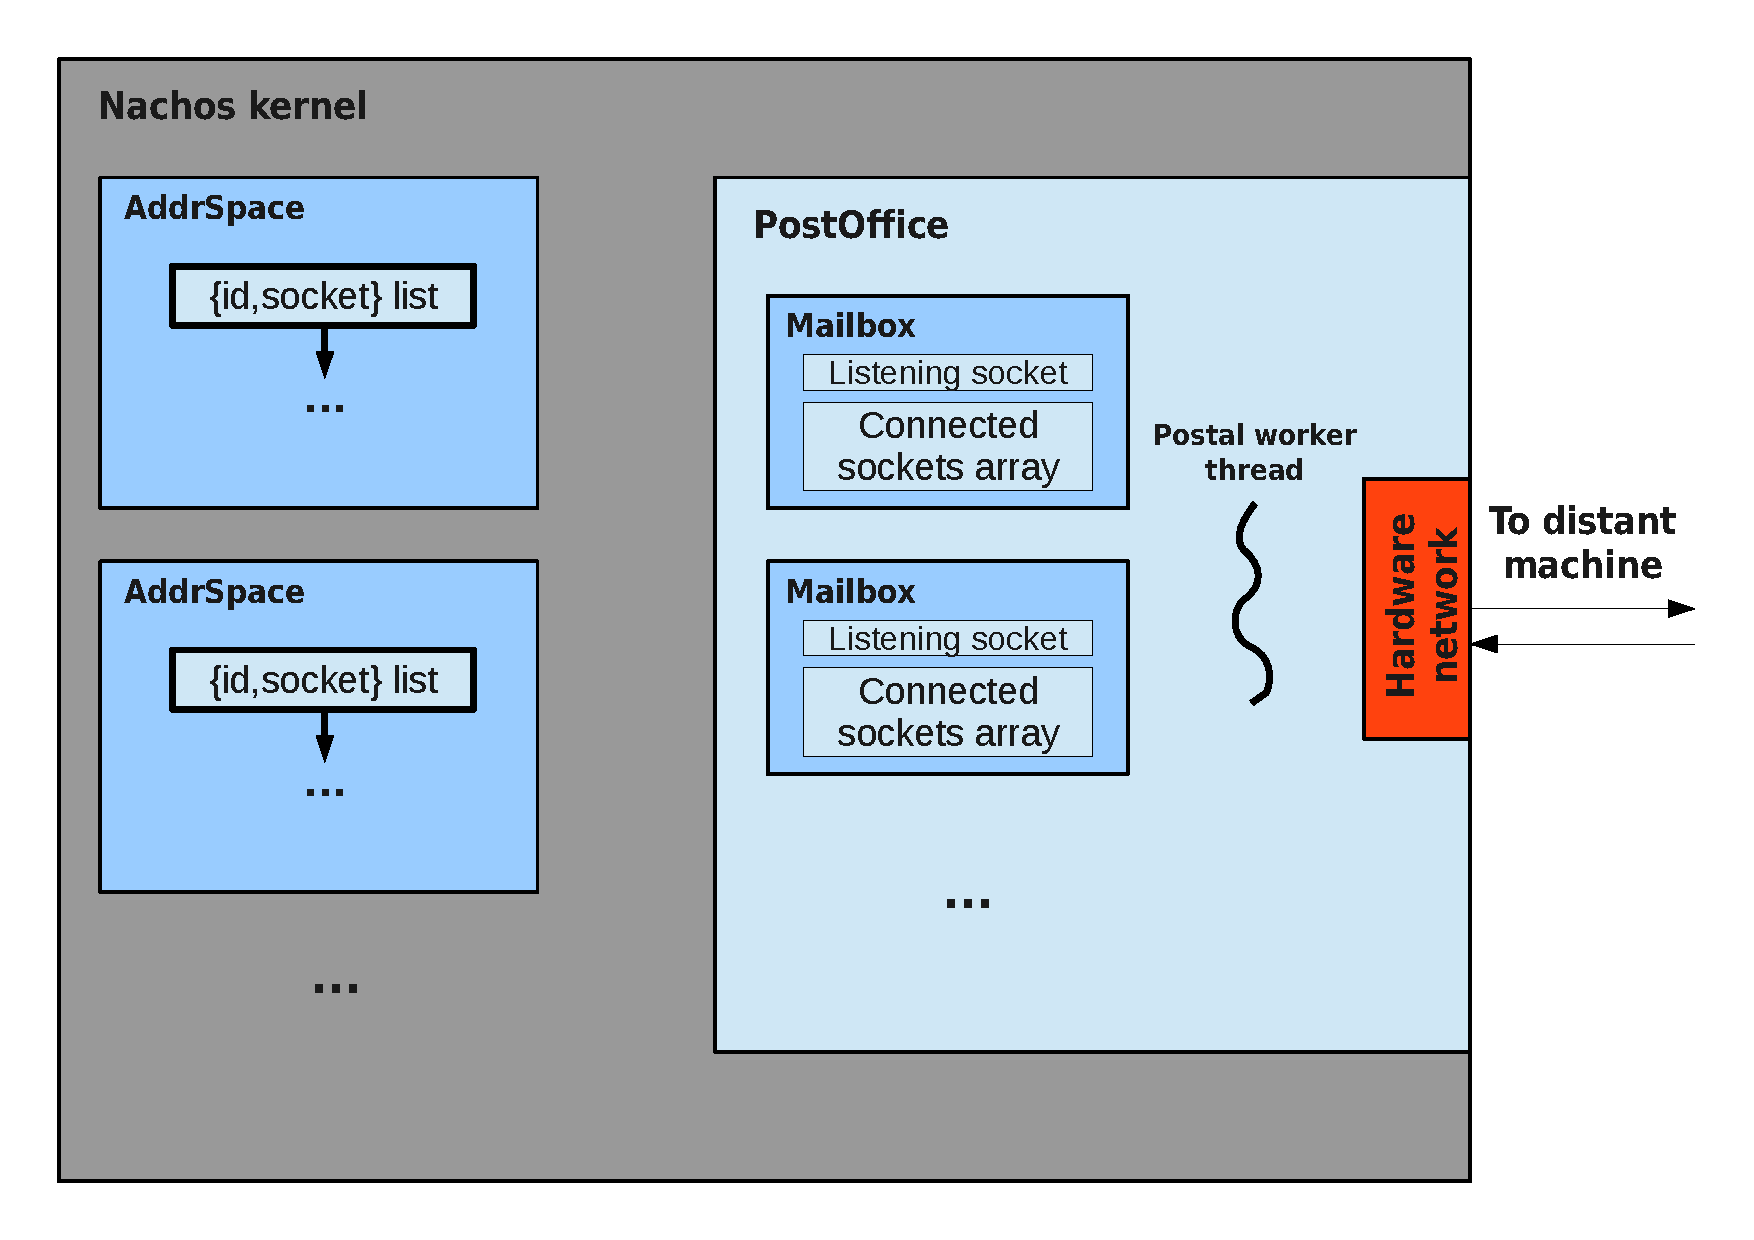
\includegraphics[width=0.7\linewidth]{Networkcolored.pdf}
    \end{figure}
  \end{itemize}
\end{frame}

\section{Quality}
\begin{frame}{Automatic Regression Test}
  \begin{itemize}
    \item Manual Test : Manually test the function per step
    \item Automatic Regression Test : Run once for every function
    \\"picture"
  \end{itemize}
\end{frame}

\begin{frame}{Memory leak prevention}
  \begin{itemize}
    \item No more memory leak
    \item System well tested
    \item No bad memory access
  \end{itemize}
\end{frame}

\section{Project Management}
\begin{frame}{Project Management}
\begin{itemize}
  \item 
  \end{itemize}
\end{frame}

\section{Conclusion}
\begin{frame}{Conclusion}
\begin{itemize}
  \item 
  \end{itemize}
\end{frame}


\end{document}

